\chapter{Literature Review}

\section{Popular Culture}

\begin{figure}[H]
\centering

\includegraphics[width=0.5\textwidth]{images/literature/rising-sun.jpg} 
\caption{Rising Sun (1993).}
\label{fig:rising-sun}
\end{figure}

\begin{figure}[H]
\centering
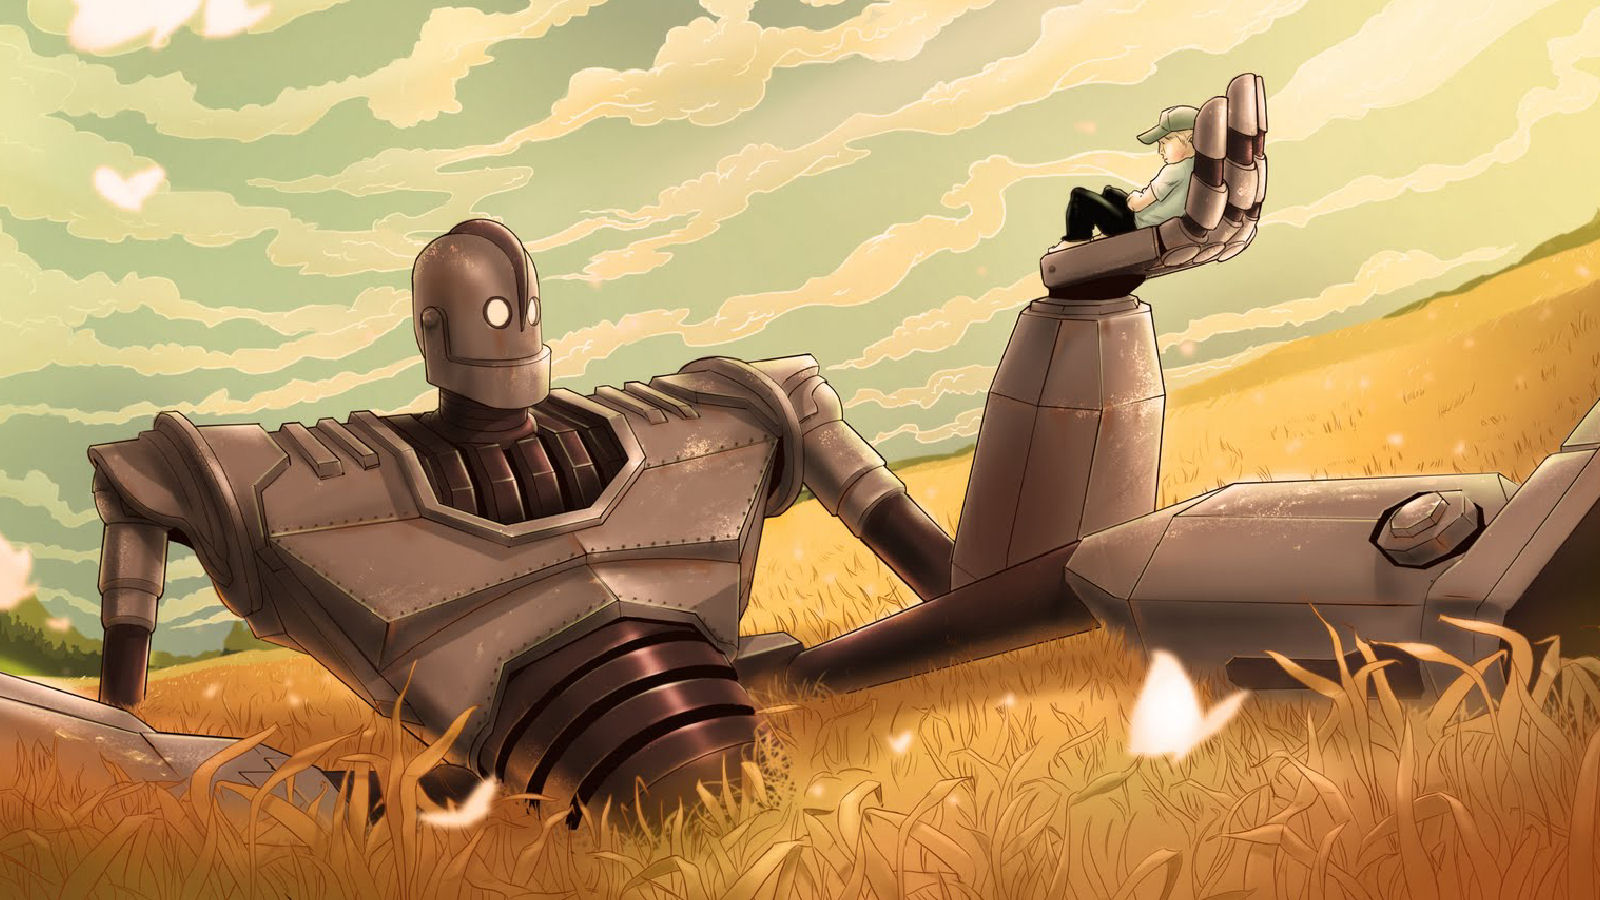
\includegraphics[width=0.5\textwidth]{images/literature/the-iron-giant-1999.jpg} 
\caption{The Iron Giant (1999).}
\label{fig:the-iron-giant-1999}
\end{figure}

\begin{figure}[H]
\centering
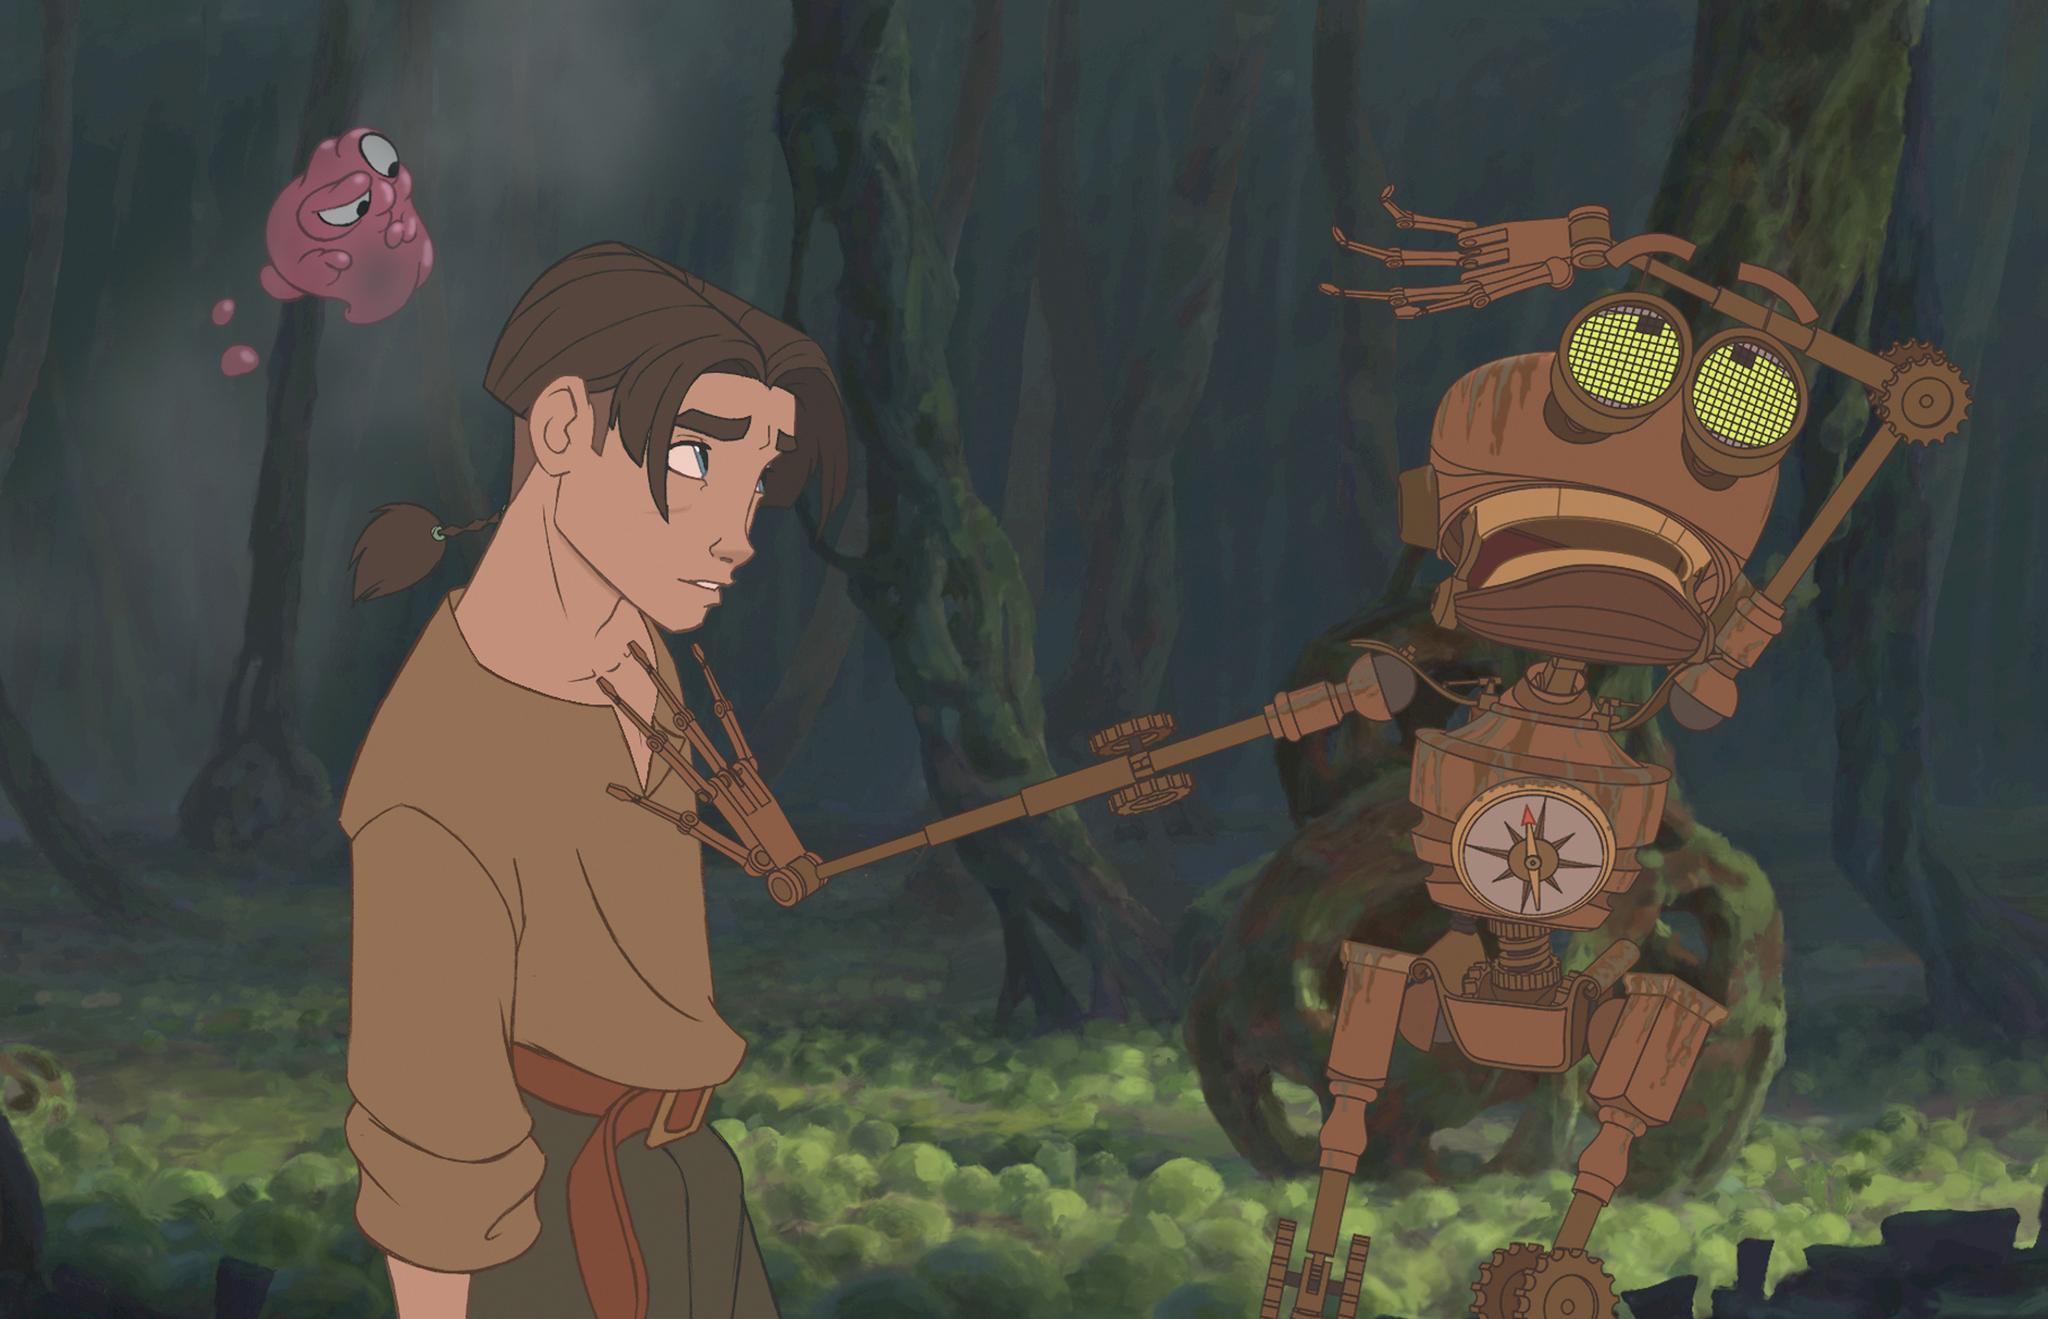
\includegraphics[width=0.5\textwidth]{images/literature/BEN-treasure-island-2002.jpg} 
\caption{Treasure Island (2002).}
\label{fig:BEN-treasure-island-2002}
\end{figure}

\section{State of the Art}

\subsection{Monoped Robots}

\begin{figure}[H]
\centering
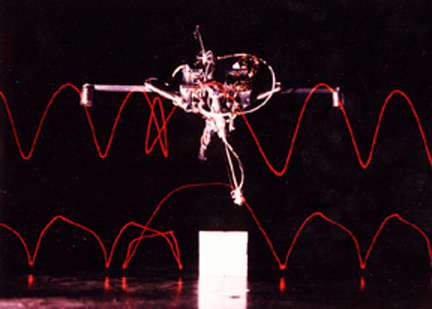
\includegraphics[width=0.5\textwidth]{images/literature/planar-one-leg-hopper.jpeg} 
\caption{Planar One-Leg Hopper - MIT Leg Laboratory (1980-1982).}
\label{fig:planar-one-leg-hopper}
\end{figure}

\begin{figure}[H]
\centering
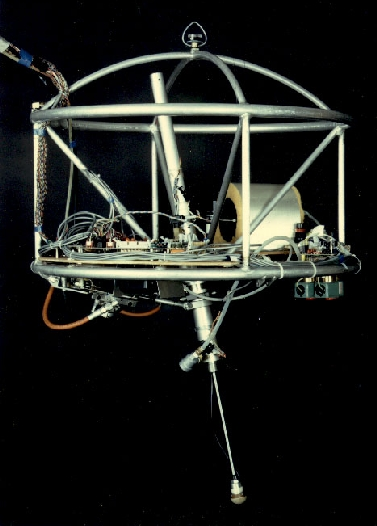
\includegraphics[width=0.5\textwidth]{images/literature/3D-one-leg-hopper.jpeg} 
\caption{3D One-Leg Hopper - MIT Leg Laboratory (1983-1984).}
\label{fig:3D-one-leg-hopper}
\end{figure}


\subsection{Biped Robots}

\begin{figure}[H]
\centering
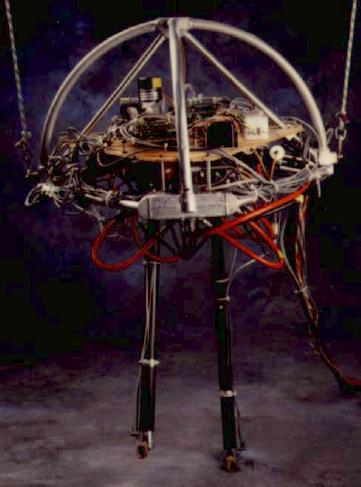
\includegraphics[width=0.5\textwidth]{images/literature/3D-biped.jpeg} 
\caption{3D Biped - MIT Leg Laboratory (1989-1995).}
\label{fig:3D-biped}
\end{figure}


\subsection{Quadruped Robots}

\begin{figure}[H]
\centering
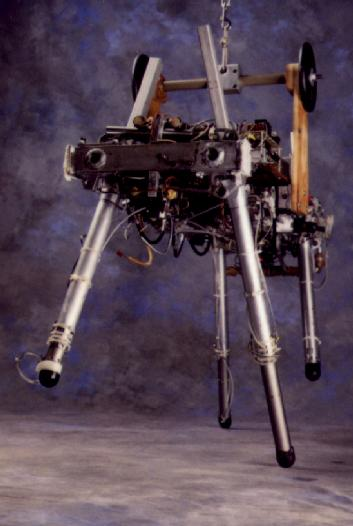
\includegraphics[width=0.5\textwidth]{images/literature/quadruped.jpeg} 
\caption{Quadruped - MIT Leg Laboratory (1984-1987).}
\label{fig:quadruped}
\end{figure}

\begin{figure}[H]
\centering
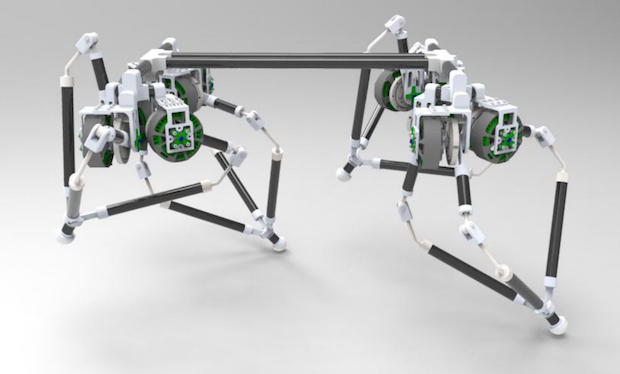
\includegraphics[width=0.5\textwidth]{images/literature/goat-leg.jpeg} 
\caption{GOAT 3-DOF Leg Topology - (Kalouche, 2016).}
\label{fig:goat-leg}
\end{figure}


\subsection{Bio-inspired Legged Robotics}

\begin{figure}[H]
\centering
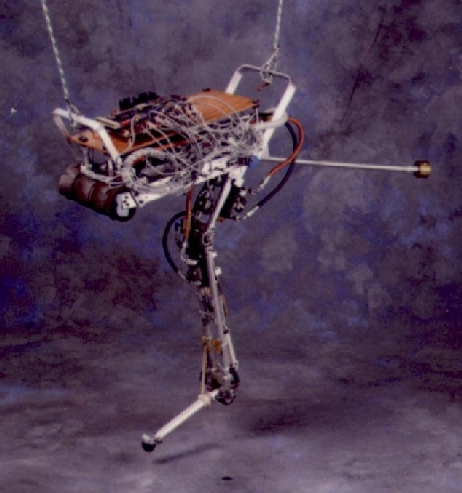
\includegraphics[width=0.5\textwidth]{images/literature/uniroo-bioinspired.jpeg} 
\caption{Uniroo - MIT Leg Laboratory (1991-1993).}
\label{fig:uniroo-bioinspired}
\end{figure}

\begin{figure}[H]
\centering
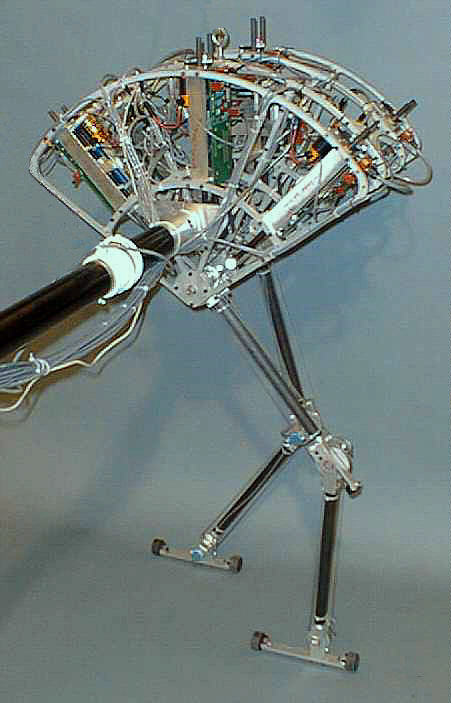
\includegraphics[width=0.5\textwidth]{images/literature/spring-flamingo.jpg} 
\caption{Spring Flamingo - MIT Leg Laboratory (1996-2000).}
\label{fig:spring-flamingo}
\end{figure}

\subsection{Humanoid Robots}

\begin{figure}[H]
\centering
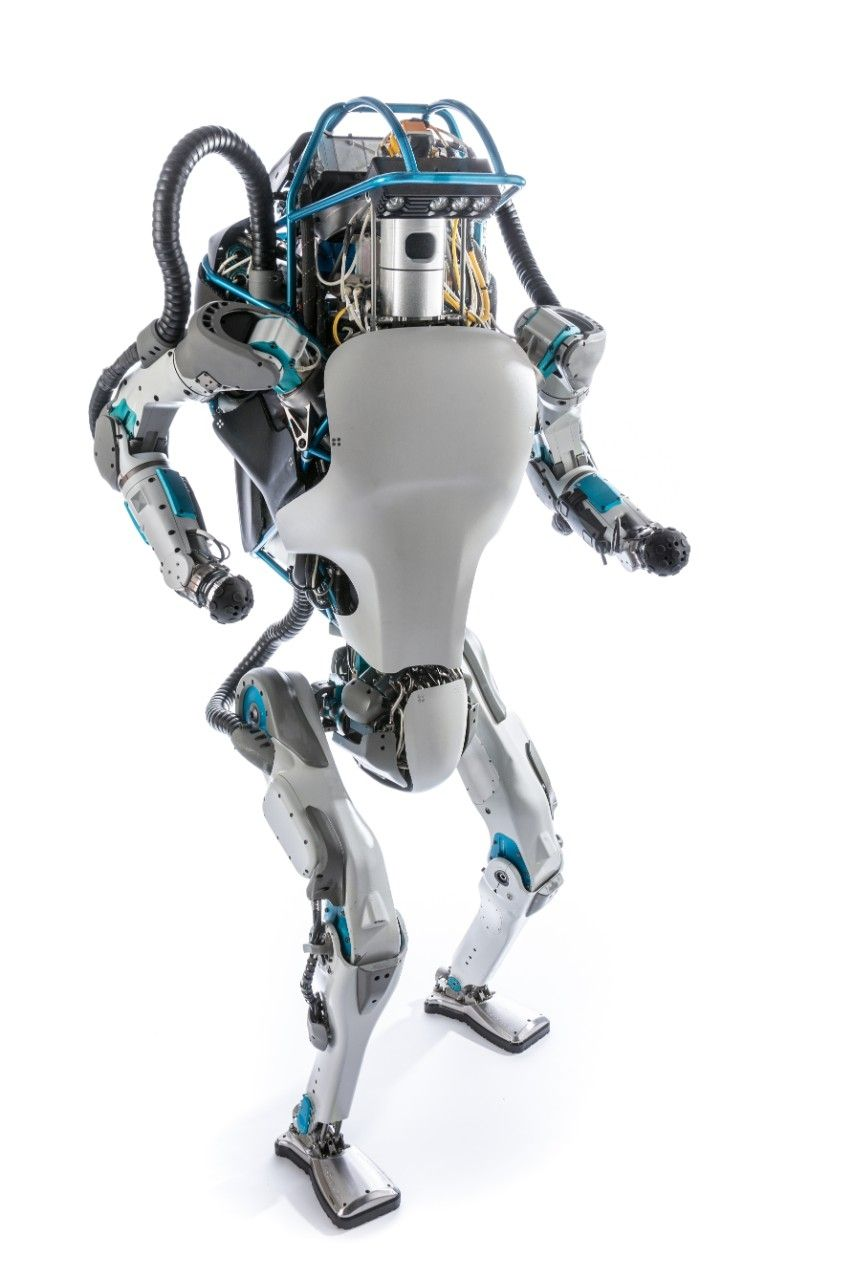
\includegraphics[width=0.5\textwidth]{images/literature/atlas-humanoid.jpg} 
\caption{Atlas Humanoid Robot - Boston Dynamics (2013).}
\label{fig:legV1}
\end{figure}

\subsection{Closed Kinematic Chain Leg}

\begin{figure}[H]
\centering
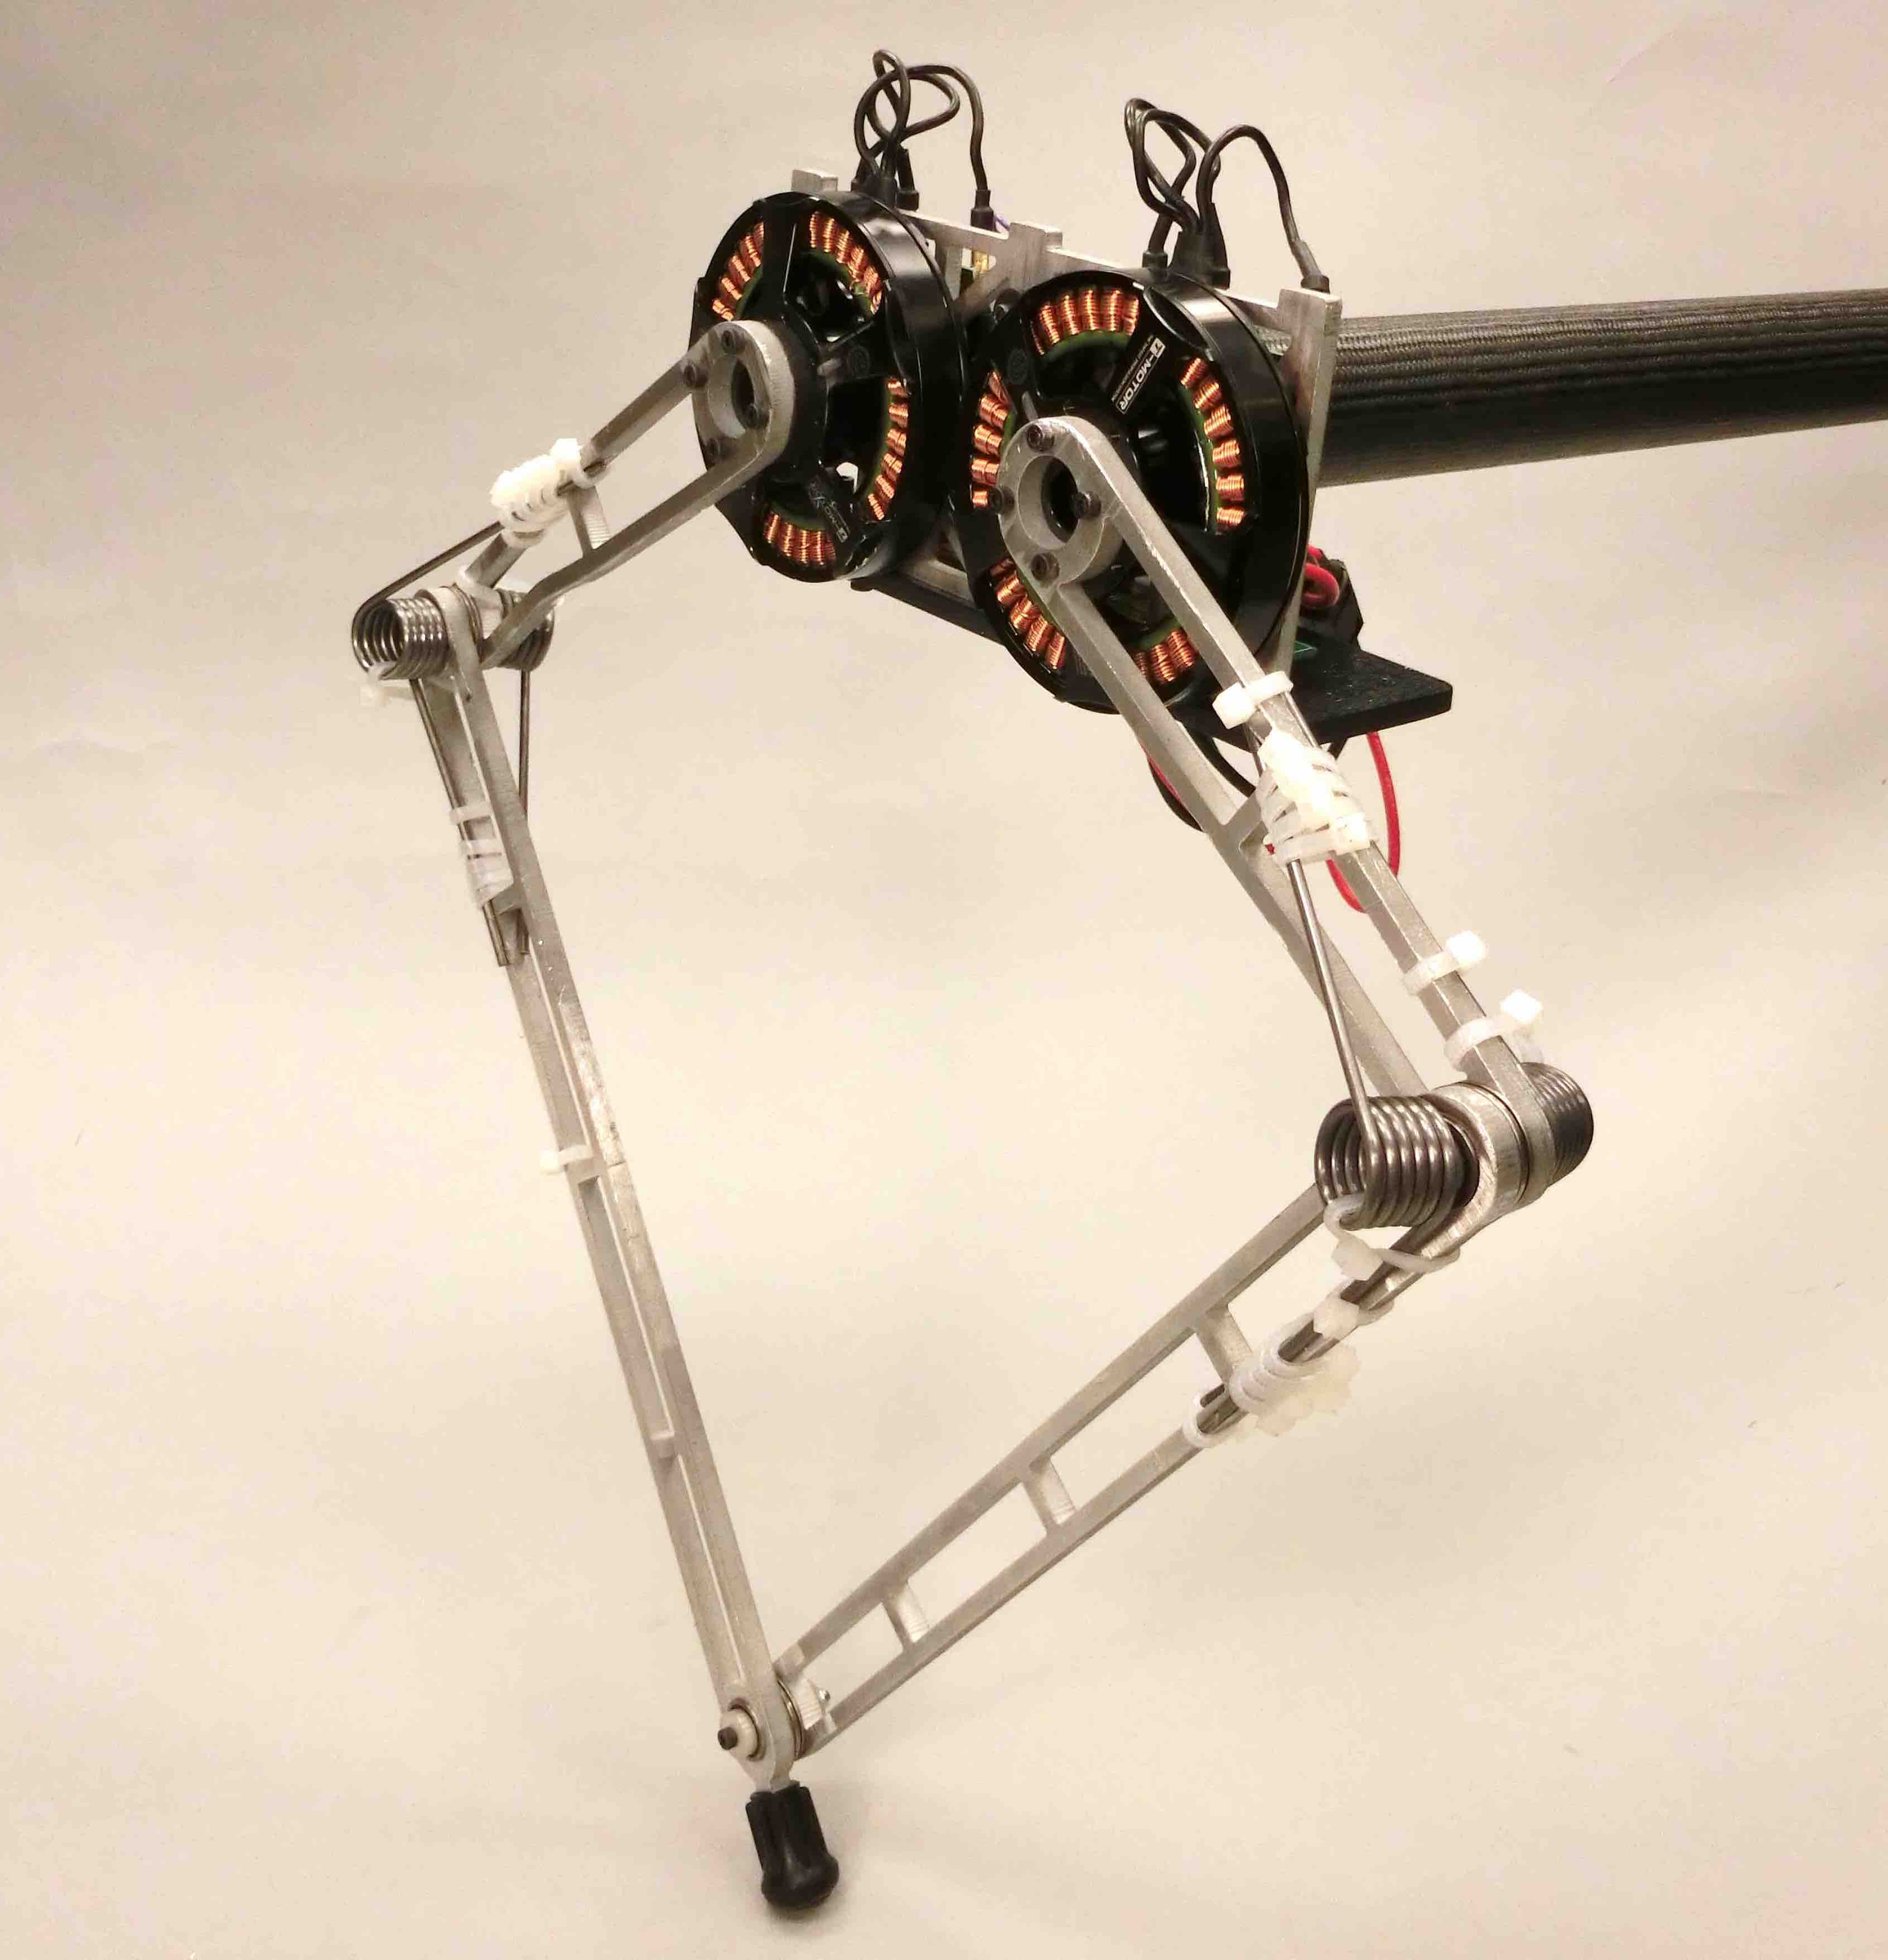
\includegraphics[width=0.5\textwidth]{images/literature/pen-state-scissor.jpg} 
\caption{Closed Kinematic Chain Leg using Raibert's Scissor Algorithm (Duperret, Koditschek, 2016).}
\label{fig:pen-state-scissor}
\end{figure}

\section{Legged Locomotion in Nature}

\section{Raibert Control}

\begin{figure}[H]
\centering
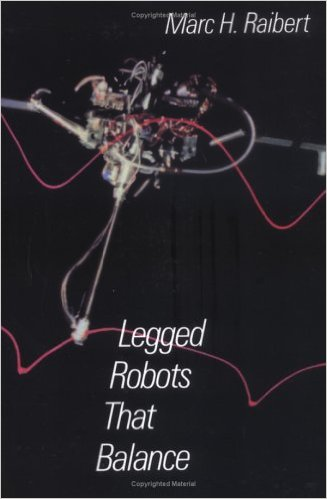
\includegraphics[width=0.5\textwidth]{images/literature/legged-robots-that-balance.jpg} 
\caption{Legged Robots That Balance - Marc H. Raibert (1986).}
\label{fig:legged-robots-that-balance}
\end{figure}

\subsection{Raibert's Scissor Algorithm}

\subsection{Phases of Motion}



\cite{Raibert1977}
\cite{Raibert1984}
\cite{Raibert1989}

\subsection{Dynamic Stability vs Static Stability}
\subsection{Phases of Motion}
\subsection{Leg Stance Control}
\section{Force Control}
